\chapter{Coexistence theory and the frequency-dependence of priority effects}
%\chaptermark{Positive frequency-dependence}
%\renewcommand{\sectionmark}[1]{}
\fancyhead[LE, RO]{\thepage}
\fancyhead[RE]{CHAPTER 3}
\fancyhead[LO]{POSITIVE FREQUENCY-DEPENDENCE}
\fancyfoot{}
\renewcommand{\headrulewidth}{0pt}
\setlength{\parindent}{1cm}


\begin{comment}
\documentclass[hidelinks,12pt]{article}
\usepackage{graphicx,bm, booktabs,lineno,array}
\usepackage[fleqn]{amsmath}
\setlength{\mathindent}{0pt}
\usepackage[super,comma,numbers, compress]{natbib}
\usepackage[a4paper]{geometry}
\usepackage[parfill]{parskip}
\usepackage[usenames,dvipsnames]{color}
\usepackage[font=footnotesize,labelfont=bf,margin=1cm, labelsep = none]{caption} 
\usepackage{setspace}
\usepackage{gensymb}
\usepackage{color} 
\usepackage{sidecap}
\usepackage{epigraph}
\usepackage{float}
\usepackage{soul,xcolor}
\setstcolor{red}
\setlength\epigraphwidth{12cm}
\setlength\epigraphrule{0pt}
\usepackage{etoolbox}
\usepackage{tcolorbox}
\tcbuselibrary{breakable}
\usepackage[bottom, symbol]{footmisc}
\usepackage{authblk}
\usepackage{hyperref}
\usepackage[color=cyan]{todonotes}
\pdfminorversion=3
\doublespacing

\renewcommand{\epigraphflush}{center}
\renewcommand{\sourceflush}{flushleft}
\newcommand{\plus}{\raisebox{.4\height}{\scalebox{.6}{+}}}
\newcommand{\minus}{\raisebox{.4\height}{\scalebox{.8}{-}}}
\renewcommand{\thefootnote}{\fnsymbol{footnote}}
\newcommand*\samethanks[1][\value{footnote}]{\footnotemark[#1]}
\newcommand\blfootnote[1]{%
  \begingroup
  \renewcommand\thefootnote{}\footnote{#1}%
  \addtocounter{footnote}{-1}%
  \endgroup
}
\end{comment}



\begin{comment}
\title{Coexistence theory and the frequency-dependence of priority effects}
\author[1]{Po-Ju Ke \thanks{Both authors contributed equally.}}
\author[1,2,3]{Andrew D. Letten \samethanks}
\affil[1]{Department of Biology, Stanford University, Stanford, California, 94305-5020, USA}
\affil[2]{Centre for Integrative Ecology, University of Canterbury, Christchurch, New Zealand}
\affil[3]{Institute of Integrative Biology, Department of Environmental Systems Science, ETH Z{\"u}rich, 8092 Z{\"u}rich, Switzerland}

\begin{document}

\date{}
\maketitle
\blfootnote{Correspondence email: pojuke@stanford.edu, andrew.letten@usys.ethz.ch}
%\textbf{Running title:} PFD
%\textbf{Keywords:} No key words for Forum 
\textbf{Type of article:} Brief Communication\\
\textbf{Number of words:} 1847 [main text] \\
\textbf{References:} 17\\
\textbf{Display items:} 3\\
\end{comment}



\section{Abstract}
Priority effects are commonly invoked to describe a broad suite of phenomena capturing the influence of species arrival order on the diversity, composition and function of ecological communities. Several studies have suggested reframing priority effects around the stabilizing and equalizing concepts of coexistence theory. We show that the only compatible priority effects are those characterized by positive frequency dependence, irrespective of whether they emerge in equilibrium or non-equilibrium systems. 



\section{Main text}
The order in which species arrive in a locality can have lasting impacts on the diversity, composition and function of ecological communities \citep{Chase2003Oecologia, Fukami2015}. This phenomenon, frequently referred to as priority effects, historical contingency or founder control \citep{Slatkin1974}, was originally explored analytically through Lotka--Volterra competition models \citep{Lewontin1969, May1971}. In these simple models, priority effects emerge when each species' growth rate is a positive function of its relative abundance, which results in the emergence of alternative stable states (panel a of Fig.~\ref{fig:FigBox}). From a theoretical perspective, the term priority effect is indeed synonymous with any process generating alternative stable states \citep{Petraitis2013}, but over time its usage has broadened to encompass a wider suite of phenomena, including those lacking multiple attractors. Several studies have subsequently mooted the prospect of reorganizing priority effects around the stabilizing and equalizing concepts of coexistence theory \citep{Mordecai2011, Fukami2016, Letten2017}. Here, we identify the unrecognized problems and promise of such an endeavour. In particular, we demonstrate that the only compatible priority effects are those characterized by positive frequency dependence. 
\par 


According to coexistence theory, species can coexist when the fitness differences between them are smaller than their niche differences, where the former compares overall adaptedness to a shared environment, and the latter captures overlap in resource usage in space and time \citep{Chesson2000}. This is equivalent to stating that each species exhibits negative frequency dependence (NFD); i.e., reduced growth as a function of its own relative abundance in a community. For a two-species Lotka--Volterra competition model, this can be summarized via the inequality 

\begin{equation}
\rho < \frac{f_{2}}{f_{1}} < 1/\rho
\tag{3.1}\label{eq:3.1}
\end{equation}

\noindent where niche overlap, $\rho$, is equal to `1 - the niche difference' and is bounded between 0 and 1, and $\frac{f_{2}}{f_{1}}$ is the fitness ratio (panel b, c of Fig.~\ref{fig:FigBox}). It follows that we can differentiate between two classes of coexistence mechanisms: equalizing mechanisms that reduce the fitness difference and stabilizing mechanisms that reduce niche overlap. 
\par


In addition to being ecologically intuitive, the bounding of niche overlap between 0 and 1 has statistical provenance in Chesson's original definition as the correlation between species' resource utilization functions in MacArthur's consumer-resource model \citep{Chesson1990}. More recently, however, Chesson provided a convenient formula for niche overlap in terms of the Lotka--Volterra competition coefficients, $\alpha_{ij}$ \citep{Chesson2013ecosys}. Specifically,

\begin{equation}
\rho=\sqrt {\frac{{{\alpha_{12}}{\alpha_{21}}}}{{{\alpha_{11}}{\alpha_{22}}}}}.
\tag{3.2}\label{eq:3.2}
\end{equation}
 
\noindent Whether or not a given $\rho$ generates NFD depends on the fitness difference between competing species, but it is clear from this formulation that $\rho$ is bounded by 0 and 1 only when the product of the intra-specific coefficients is greater than the product of the inter-specific coefficients. When the reverse is true, $\rho$ takes values greater than 1, and the system exhibits priority effects giving rise to two alternative stable states, depending on species' initial density (panel a, b of Fig.~\ref{fig:FigBox}). 
\par


At first glance, $\rho>1$ is at odds with both intuitive and statistical interpretations of niche overlap, and seemingly becomes even more nonsensical when cast as a negative niche difference (1 - $\rho$). However, this break with convention operationalizes the criteria for positive frequency dependence (PFD), i.e., the analytical definition of priority effects, as the inverse of the stable coexistence inequality (panel b of Fig.~\ref{fig:FigBox}): 

\begin{equation}
\rho > \frac{f_{2}}{f_{1}} > 1/\rho.
\tag{3.3}\label{eq:3.3}
\end{equation}

\noindent Now, if we rename the niche difference ($1-\rho$) as the stabilization potential to avoid the semantic challenges of referring to a negative niche difference, we see from Eqn.~\ref{eq:3.3} that any mechanism that reduces the fitness ratio, or further decreases the stabilization potential below zero (i.e., further increases $\rho$ above one), will increase the probability of priority effects. Thus, like stable coexistence, we recognize that stable priority effects are also jointly controlled by both stabilizing and equalizing mechanisms. Note that the stabilization potential diverges around zero such that values above zero represent the stabilization potential for coexistence, whereas values below zero represent the stabilization potential for priority effects; in other words the strength of the attractor towards alternative stable states (panel b of Fig.~\ref{fig:FigBox}). Our terminology is different from recent heuristic translations of priority effects into coexistence theory, where the decrease of niche differences (i.e., stabilization potential) below zero has been referred to as destabilization \citep{Mordecai2011, Fukami2016}. However, while the coexistence attractor becomes unstable, multiple community attractors arise to be dynamically stable. Therefore, we favor conceptualizing destabilization as any process that causes the stabilization potential to approach zero from values above \textit{or} below (Fig. 1e). 
\par
 
 
A classic example of priority effects emerging from PFD comes from Tilman's 1982 monograph \cite{tilman1982}. Using the approach taken by Letten \textit{et al}.\cite{Letten2017} to derive niche overlap and the fitness ratio from Tilman's consumer-resource model, PFD generated priority effects can be partitioned into stabilizing and equalizing components. This partitioning is achieved by translating Tilman's model into a Lotka--Volterra form, which allows for the derivation of competition coefficients in terms of consumer-resource parameters. From there we can explore the effect of modifying mechanistic parameters on the stabilization potential using Eqn.~\ref{eq:3.2}, and the fitness ratio using the companion formula \citep{Chesson2008b, Chesson2013ecosys} (full derivation provided in Appendix B):

\begin{equation}
\frac{f_{2}}{f_{1}}=\sqrt {\frac{{{a_{11}}{a_{12}}}}{{{a_{22}}{a_{21}}}}}.
\tag{3.4}\label{eq:3.4}
\end{equation}

\noindent In Figure 1a, NFD and coexistence arise due to a combination of: 1) intersecting zero net growth isoclines (ZNGIs)\footnote{Zero net growth isocline (ZNGI) = the set of resource concentrations at which species' growth balances mortality. Consumption vectors = relative rates at which resources are depleted via consumption. Resource supply point = resource availability the system would return to in the absence of consumption.} indicating a trade-off in the two species competitive fitness for two substitutable resources where the red species benefits more from $R_{2}$ and the blue species from $R_{1}$; 2) consumption vectors that are directed towards each species' favored resource, such that the red species consumes more of $R_{2}$ and vice-versa, which is a prerequisite for intra-specific feedbacks being greater than inter-specific feedbacks; and 3) an intermediate resource ratio, which ensures neither species is overly advantaged by an imbalanced abundance of their favoured resource \citep{Chase2003, Letten2017}. As the angle between the consumption vectors declines to $\theta_{2}$ (Fig. 1b), the stabilization potential also declines. The outcome is competitive exclusion when the stabilization potential falls below the fitness ratio (Fig. 1e). Once the consumption vectors cross and begin to diverge, each species consumes more of its competitor's favored resource ($\theta_{3}$, Fig. 1c), setting up the conditions for PFD. However, if the fitness difference remains sufficiently large, the outcome will still be exclusion irrespective of arrival order (Fig. 1e). If the resource supply shifts to a more balanced ratio (Fig. 1d), the fitness inequality is reduced and priority effects emerge (Fig. 1e). The species that arrives first reduces the resource level of its competitors favoured resource below the competitor's $R^*$ - the minimum resource concentration required to maintain a positive growth rate, denoted by the intercept of the ZNGI with the resource axis. The result is that the late arriving competitor is unable to invade. 
\par


The above results demonstrate that priority effects are a function of both the stabilization potential and the fitness inequality, and that only a subset of phenomena commonly referred to as priority effects are compatible with coexistence theory. In particular, compatible phenomena are limited to those that generate PFD and therefore are consistent with the original definition derived from Lotka--Volterra \citep{Petraitis2013}. This is not to say that PFD is unique to systems exhibiting point equilibria. For example, the coexistence-affecting mechanism relative nonlinearity can generate PFD when species that benefit from fluctuations in the intensity of competition also exacerbate those fluctuations \citep{Chesson2009}. In Figure 2, two species with nonlinear functional responses exhibit negative average invader growth rates when competing for a logistically growing resource. As the resident, blue is able to draw resource levels below red's $R^*$ and therefore prevent red from invading, whereas, at sufficiently high initial density, red generates large resource fluctuations which blue is unable to control. Nevertheless, in a system that precludes the emergence of positive (or negative) frequency dependence, and hence the emergence of a non-zero stable attractor, the stabilization potential term is unquantifiable. This criterion, however, wholly or partially excludes a number of phenomena lacking multiple attractors, which for heuristic reasons are often included under the umbrella of priority effects (see examples in Fukami \cite{Fukami2015}). We briefly consider two of these phenomena below. 
\par


%\subsection*{Positive density dependence and facilitation}
When applying coexistence theory to study priority effects, it is important to recognize that PFD can emerge from negative or positive density dependence, i.e., facilitation. However, while Eqn.~\ref{eq:3.2}) cannot be leveraged to interpret the facilitative dynamics since negative $\alpha_{ij}$ in the Lotka--Volterra framework would generate unbounded population densities. Facilitation, of course, cannot go on forever and coexistence theory may still provide insight when negative density dependence starts to operate \citep{Schreiber2017}. However, unless constrained by specific model designs, the formulas can only be applied to PFD emerging from negative density dependence. 
\par


An alternative form of positive density dependence sometimes characterized as a priority effects is an Allee effect \citep{Petraitis2013}. For species exhibiting an Allee effect, there is a density threshold dividing two alternative stable states, i.e., above which the population persists and below which the population goes extinct. As such the alternative stable states arise from endogenous mechanisms at the population level, and therefore are distinct from priority effects that emerge at the community level driven by species interactions. Thus, while Allee effects can effect community composition if inter-specific interactions maintain species below their Allee threshold, they arise independently of a species' frequency in a community. 
\par


%\subsection*{Succession and transient priority effects}
Finally, the notion of priority effects has also been usefully applied to understand the effects of arrival order on successional dynamics. In these instances, differences in initial abundance can cause compositional trajectories to vary through time, even though they may all eventually converge on the same community state. Such ``alternative transient states" \citep{FukamiNakajima2011} can also be observed in naturally ephemeral microbial systems, such as those that develop in floral nectar or woody debris, where the final state might be the local extinction of all community members following the exhaustion of available resources. The trajectories of these communities, which are an outcome of resource pre-emption, may have downstream impacts on pollinator preference and decomposition rates and therefore undoubtedly reflect ecological phenomena with meaningful consequences for ecosystem function. Furthermore, it may well be relevant to consider these processes with respect to stabilizing mechanisms operating at some larger temporal or spatial scales. Nevertheless, treated independently of their broader spatio-temporal context, there is little scope or rationale to bring coexistence theory to bear on such phenomena. 
\par


%\subsection*{Summary}
Interest in coexistence theory has been growing steadily, but to date the overwhelming emphasis has been on the underlying stabilizing mechanisms giving rise to NFD and stable coexistence. We have illustrated the most accessible approach to incorporating priority effects mediated through PFD into this body of theory. When priority effects emerge from positive density dependence, or arise in transient systems, it is currently unclear how to analytically connect them to coexistence theory. 
\par



\section{Methods}
\subsection{Positive frequency dependence in an equilibrium system}
We first provide an example of positive frequency dependence (PFD) emerging from resource competition in an equilibrium system (Fig. 1). To this end, we take Tilman's original consumer-resource model \citep[p.~270]{tilman1982}, where two consumers (i.e. $N_{1}$ and $N_{2}$) are competing for two perfectly substitutable resources, $R_{1}$ and $R_{2}$. The dynamics of this system can be described as follows:

\begin{equation}
\frac{{d{N_1}}}{{dt}} = {r_1}{N_1}\left[ {\frac{{{w_{11}}{R_1} + {w_{12}}{R_2} - {T_1}}}{{{k_1} + {w_{11}}{R_1} + {w_{12}}{R_2} - {T_1}}}} \right] - D{N_1} \tag{3.7}\label{eq:3.7}
\end{equation}
\begin{equation}
\frac{{d{N_2}}}{{dt}} = {r_2}{N_2}\left[ {\frac{{{w_{21}}{R_1} + {w_{22}}{R_2} - {T_2}}}{{{k_2} + {w_{21}}{R_1} + {w_{22}}{R_2} - {T_2}}}} \right] - D{N_2} \tag{3.8}\label{eq:3.8}
\end{equation}
\begin{equation}
\frac{{d{R_1}}}{{dt}} = D\left( {{S_1} - {R_1}} \right) - {c_{11}}{N_1} - {c_{21}}{N_2} \tag{3.9}\label{eq:3.9}
\end{equation}
\begin{equation}
\frac{{d{R_2}}}{{dt}} = D\left( {{S_2} - {R_2}} \right) - {c_{12}}{N_1} - {c_{22}}{N_2} \tag{3.10}\label{eq:3.10}
\end{equation}

Here, $r_{i}$ represents the maximum population growth rate for species $i$ ($i = $ 1 or 2) and $D$ represents the constant mortality of the consumers and turnover rate of resources. Per capita resource consumption rate of consumer $N_{i}$ on resource $R_{j}$ ($j = $ 1 or 2) is represented by $c_{ij}$, whereas $w_{ij}$ represents a weighting factor that converts availability of $R_{j}$ into its value for consumer $N_{i}$. Following a Monod growth model, $k_{i}$ is the half-saturation constant for $N_{i}$ resource consumption, and $T_{i}$ is the minimum amount of total resource required for $N_{i}$ to grow. Finally, $S_{1}$ and $S_{2}$ represent the resource supply concentrations for $R_{1}$ and $R_{2}$, respectively. For this model, we define the consumption vectors for consumer $i$ on the two substitutable resources as a vector with elements $\left( c_{i1}, c_{i2} \right)$, and the supply point can be expressed as a point with coordinates $\left( S_{1}, S_{2} \right)$. 
\par


We used the approach implemented in Letten \textit{et al.}\citep{Letten2017} to translate changes in the parameters of Tilman's consumer-resource model \citep{tilman1982} into changes to the stabilization potential (1 - $\rho$) and fitness ratio ($\frac{f_{2}}{f_{1}}$) of coexistence theory (see Appendix B for detail mathematical treatment). In brief, we solved the coexistence equilibrium of a consumer-resource model and rearrange it algebraically to a form that is comparable to the equilibrium of a two species Lotka--Volterra competition model (i.e., Eqns.~\ref{eq:LV1} and \ref{eq:LV2} in Box 1). We then quantified the stabilization potential and fitness ratio based on equations in the main text. For our specific model, we can express these two components of coexistence theory as follows: 

\begin{equation}
\rho  = \sqrt {\frac{{{a_{12}}{a_{21}}}}{{{a_{11}}{a_{22}}}}}  = \sqrt {\frac{\left (
		c_{22} + c_{21}\frac{w_{11}}{w_{12}}\right )\left ( 
		c_{12} + c_{11}\frac{w_{21}}{w_{22}} \right )}{\left (
		c_{12} + c_{11}\frac{w_{11}}{w_{12}}\right )\left ( 
		c_{22} + c_{21}\frac{w_{21}}{w_{22}} \right )}}
\tag{3.11}\label{eq:3.11}
\end{equation}
\begin{equation}
\frac{{{f_2}}}{{{f_1}}} = \sqrt {\frac{{{a_{11}}{a_{12}}}}{{{a_{22}}{a_{21}}}}}  = \frac{\left (S_{2}+\frac{w_{21}}{w_{22}}S_{1}-B_{2}\right )}{\left (S_{2}+\frac{w_{11}}{w_{12}}S_{1}-B_{1}\right )}\sqrt {\frac{\left (
				c_{12} + c_{11}\frac{w_{11}}{w_{12}}\right )\left ( 
				c_{22} + c_{21}\frac{w_{11}}{w_{12}} \right )}{\left (
				c_{22} + c_{21}\frac{w_{21}}{w_{22}}\right )\left ( 
				c_{12} + c_{11}\frac{w_{21}}{w_{22}} \right )}}
\tag{3.12}\label{eq:3.12}
\end{equation} 
				
where 

\begin{equation}
{B_1} = \left[ {\frac{{D\left( {{k_1} - {T_1}} \right) + {r_1}{T_1}}}{{{w_{12}}\left( {{r_1} - D} \right)}}} \right]
\tag{3.13}\label{eq:3.13}
\end{equation} 
\begin{equation}
{B_2} = \left[ {\frac{{D\left( {{k_2} - {T_2}} \right) + {r_2}{T_2}}}{{{w_{21}}\left( {{r_2} - D} \right)}}} \right]\left( {\frac{{{w_{21}}}}{{{w_{22}}}}} \right).
\tag{3.14}\label{eq:3.14}
\end{equation} 

\noindent We varied species' per capita consumption rates, $c_{ij}$, and the supply point to study the effects of changing consumer-resource parameters on stabilization potential and fitness ratio. See Appendix B for detailed parameter values. 
\par
	
				
				
\subsection{Positive frequency dependence in an non-equilibrium system}
Next, we provide an example of PFD emerging through the coexistence-affecting mechanism relative nonlinearity. In this example, our model consists of two consumers competing for a single logistically-growing resource. One species has a type 3 functional response (blue in Fig. 2), given by: 
				
\begin{equation}
\frac{dN_{1}}{dt} = N_{1}(\mu _{max_{1}}\frac{R^2}{Ks_{1} + R^2}-d).\tag{3.15}\label{eq:3.15}
\end{equation}
				
The other species (red in Fig. 2) has a modified Monod (type 2) functional response with inhibition at high resource levels: 
				
\begin{equation}
\frac{dN_{2}}{dt} = N_{2}(\mu _{max_{2}}\frac{R}{Ks_{2} + R + \frac{R^2}{Ki}}-d).\tag{3.16}\label{eq:3.16}
\end{equation}
				
Here, $N_{i}$ is the population density of consumer $i$ ($i = $ 1 or 2), $\mu_{max_{i}}$ is the maximum growth rate, $Ks_{i}$ is the half saturation constant, $R$ is the density/concentration of resource, $d$ is the density independent mortality rate, and $Ki$ is the inhibition term unique to the second species. 
\par


Time series simulations were run with the LSODA solver using the deSolve package v1.20 \citep{soetaert2016package} in R v3.4.2. To study PFD, we started the simulation with different initial population sizes. See Appendix B for detailed parameter values. 
\par

				
%\subsection*{Data and code availability}
%All code used for this study are available at https://github.com/pojuke/CoexistPFD and are available on request.


\begin{comment}
\newpage
%\bibliographystyle{nature}
\begin{thebibliography}{10}
\expandafter\ifx\csname url\endcsname\relax
\def\url#1{\texttt{#1}}\fi
\expandafter\ifx\csname urlprefix\endcsname\relax\def\urlprefix{URL }\fi
\providecommand{\bibinfo}[2]{#2}
\providecommand{\eprint}[2][]{\url{#2}}
	
\bibitem{Chase2003Oecologia}
	\bibinfo{author}{Chase, J.~M.}
	\newblock \bibinfo{title}{Community assembly: when should history matter?}
	\newblock \emph{\bibinfo{journal}{Oecologia}} \textbf{\bibinfo{volume}{136}},
	\bibinfo{pages}{489--498} (\bibinfo{year}{2003}).
	
\bibitem{Fukami2015}
	\bibinfo{author}{Fukami, T.}
	\newblock \bibinfo{title}{Historical contingency in community assembly:
		integrating niches, species pools, and priority effects}.
	\newblock \emph{\bibinfo{journal}{Annu. Rev. Ecol. Evol. Syst.}}
	\textbf{\bibinfo{volume}{46}}, \bibinfo{pages}{1--23} (\bibinfo{year}{2015}).
	
\bibitem{Slatkin1974}
	\bibinfo{author}{Slatkin, M.}
	\newblock \emph{\bibinfo{journal}{Ecology}} \textbf{\bibinfo{volume}{55}},
	\bibinfo{pages}{128--134} (\bibinfo{year}{1974}).
	
\bibitem{Lewontin1969}
	\bibinfo{author}{Lewontin, R.~C.}
	\newblock \bibinfo{title}{The meaning of stability.}
	\newblock In \emph{\bibinfo{booktitle}{Brookhaven symposia in biology}},
	vol.~\bibinfo{volume}{22}, \bibinfo{pages}{13} (\bibinfo{year}{1969}).
	
\bibitem{May1971}
	\bibinfo{author}{May, R.~M.}
	\newblock \bibinfo{title}{Stability in multispecies community models}.
	\newblock \emph{\bibinfo{journal}{Mathematical Biosciences}}
	\textbf{\bibinfo{volume}{12}}, \bibinfo{pages}{59--79}
	(\bibinfo{year}{1971}).
	
\bibitem{Petraitis2013}
	\bibinfo{author}{Petraitis, P.}
	\newblock \emph{\bibinfo{title}{Multiple stable states in natural ecosystems}}
	(\bibinfo{publisher}{OUP Oxford}, \bibinfo{year}{2013}).
	
\bibitem{Mordecai2011}
	\bibinfo{author}{Mordecai, E.~A.}
	\newblock \bibinfo{title}{{Pathogen impacts on plant communities: unifying
			theory, concepts, and empirical work}}.
	\newblock \emph{\bibinfo{journal}{Ecol. Monograph}}
	\textbf{\bibinfo{volume}{81}}, \bibinfo{pages}{429--441}
	(\bibinfo{year}{2011}).
	
\bibitem{Fukami2016}
	\bibinfo{author}{Fukami, T.}, \bibinfo{author}{Mordecai, E.~A.} \&
	\bibinfo{author}{Ostling, A.}
	\newblock \bibinfo{title}{A framework for priority effects}.
	\newblock \emph{\bibinfo{journal}{Journal of Vegetation Science}}
	\textbf{\bibinfo{volume}{27}}, \bibinfo{pages}{655--657}
	(\bibinfo{year}{2016}).
	
\bibitem{Letten2017}
	\bibinfo{author}{Letten, A.~D.}, \bibinfo{author}{Ke, P.-J.} \&
	\bibinfo{author}{Fukami, T.}
	\newblock \bibinfo{title}{Linking modern coexistence theory and contemporary
		niche theory}.
	\newblock \emph{\bibinfo{journal}{Ecological Monographs}}
	\textbf{\bibinfo{volume}{87}}, \bibinfo{pages}{161--177}
	(\bibinfo{year}{2017}).
	
\bibitem{Chesson2000}
	\bibinfo{author}{Chesson, P.}
	\newblock \bibinfo{title}{{Mechanisms of maintenance of species diversity}}.
	\newblock \emph{\bibinfo{journal}{Annu. Rev. Ecol. Syst.}}
	\textbf{\bibinfo{volume}{31}}, \bibinfo{pages}{343--366}
	(\bibinfo{year}{2000}).
	
\bibitem{Chesson1990}
	\bibinfo{author}{Chesson, P.}
	\newblock \bibinfo{title}{{MacArthur's consumer-resource model}}.
	\newblock \emph{\bibinfo{journal}{Theor. Popul. Biol.}}
	\textbf{\bibinfo{volume}{37}}, \bibinfo{pages}{26--38}
	(\bibinfo{year}{1990}).
	
\bibitem{Chesson2013ecosys}
	\bibinfo{author}{Chesson, P.}
	\newblock \bibinfo{title}{{Species Competition and Predation}}.
	\newblock In \bibinfo{editor}{Leemans, R.} (ed.)
	\emph{\bibinfo{booktitle}{Ecological Systems}}, \bibinfo{pages}{223--256}
	(\bibinfo{publisher}{Springer New York}, \bibinfo{year}{2013}).
	
\bibitem{tilman1982}
	\bibinfo{author}{Tilman, D.}
	\newblock \emph{\bibinfo{title}{Resource Competition and Community Structure.
			(Mpb-17)}} (\bibinfo{publisher}{Princeton University Press, Princeton, NJ,
		USA}, \bibinfo{year}{1982}).
	
\bibitem{Chesson2008b}
	\bibinfo{author}{Chesson, P.} \& \bibinfo{author}{Kuang, J.~J.}
	\newblock \bibinfo{title}{{The interaction between predation and competition.}}
	\newblock \emph{\bibinfo{journal}{Nature}} \textbf{\bibinfo{volume}{456}},
	\bibinfo{pages}{235--8} (\bibinfo{year}{2008}).
	
\bibitem{Chase2003}
	\bibinfo{author}{Chase, J.} \& \bibinfo{author}{Leibold, M.}
	\newblock \emph{\bibinfo{title}{{Ecological Niches: Linking Classical and
				Contemporary Approaches}}} (\bibinfo{publisher}{University of Chicago Press},
	\bibinfo{address}{Chicago, IL}, \bibinfo{year}{2003}).
	
\bibitem{Chesson2009}
	\bibinfo{author}{Chesson, P.}
	\newblock \bibinfo{title}{{Scale transition theory with special reference to
			species coexistence in a variable environment}}.
	\newblock \emph{\bibinfo{journal}{Journal of Biological Dynamics}}
	\textbf{\bibinfo{volume}{3}}, \bibinfo{pages}{149--163}
	(\bibinfo{year}{2009}).
	
\bibitem{Schreiber2017}
	\bibinfo{author}{Schreiber, S.}, \bibinfo{author}{Yamamichi, M.}, \& \bibinfo{author}{Strauss, S.}
	\newblock \bibinfo{title}{When rarity has costs: coexistence under positive frequency-dependence and environmental stochasticity}.
	\newblock \emph{\bibinfo{journal}{bioRxiv}}
	\textbf{\bibinfo{volume}{161919}}
	(\bibinfo{year}{2017}).

\bibitem{FukamiNakajima2011}
	\bibinfo{author}{Fukami, T.} \& \bibinfo{author}{Nakajima, M.}
	\newblock \bibinfo{title}{Community assembly: alternative stable states or
		alternative transient states?}
	\newblock \emph{\bibinfo{journal}{Ecology Letters}}
	\textbf{\bibinfo{volume}{14}}, \bibinfo{pages}{973--984}
	(\bibinfo{year}{2011}).
	
\bibitem{soetaert2016package}
	Soetaert, K. \emph{et~al.} (2016) Package ‘desolve’		
\end{thebibliography}
\end{comment}



\section{Acknowledgements}
We thank Tad Fukami, Tess Grainger, Daniel Stouffer and two anonymous reviewers for helpful comments. P.-J.K. is supported by Stanford University and the Studying Abroad Scholarship from the Ministry of Education, Taiwan. A.D.L. was supported by postdoctoral fellowship from the Center for Computational, Evolutionary, and Human Genomics of Stanford University.



%\subsection*{Author contributions}
%P.-J.K. and A.D.L. conceived the study, performed the analysis and wrote the manuscript. 



%\subsection*{Competing interests}
%The authors declare no competing financial interests.



\newpage
\section{Figures}
\begin{figure}[h!]
	\centering
	\makebox[\textwidth][c]{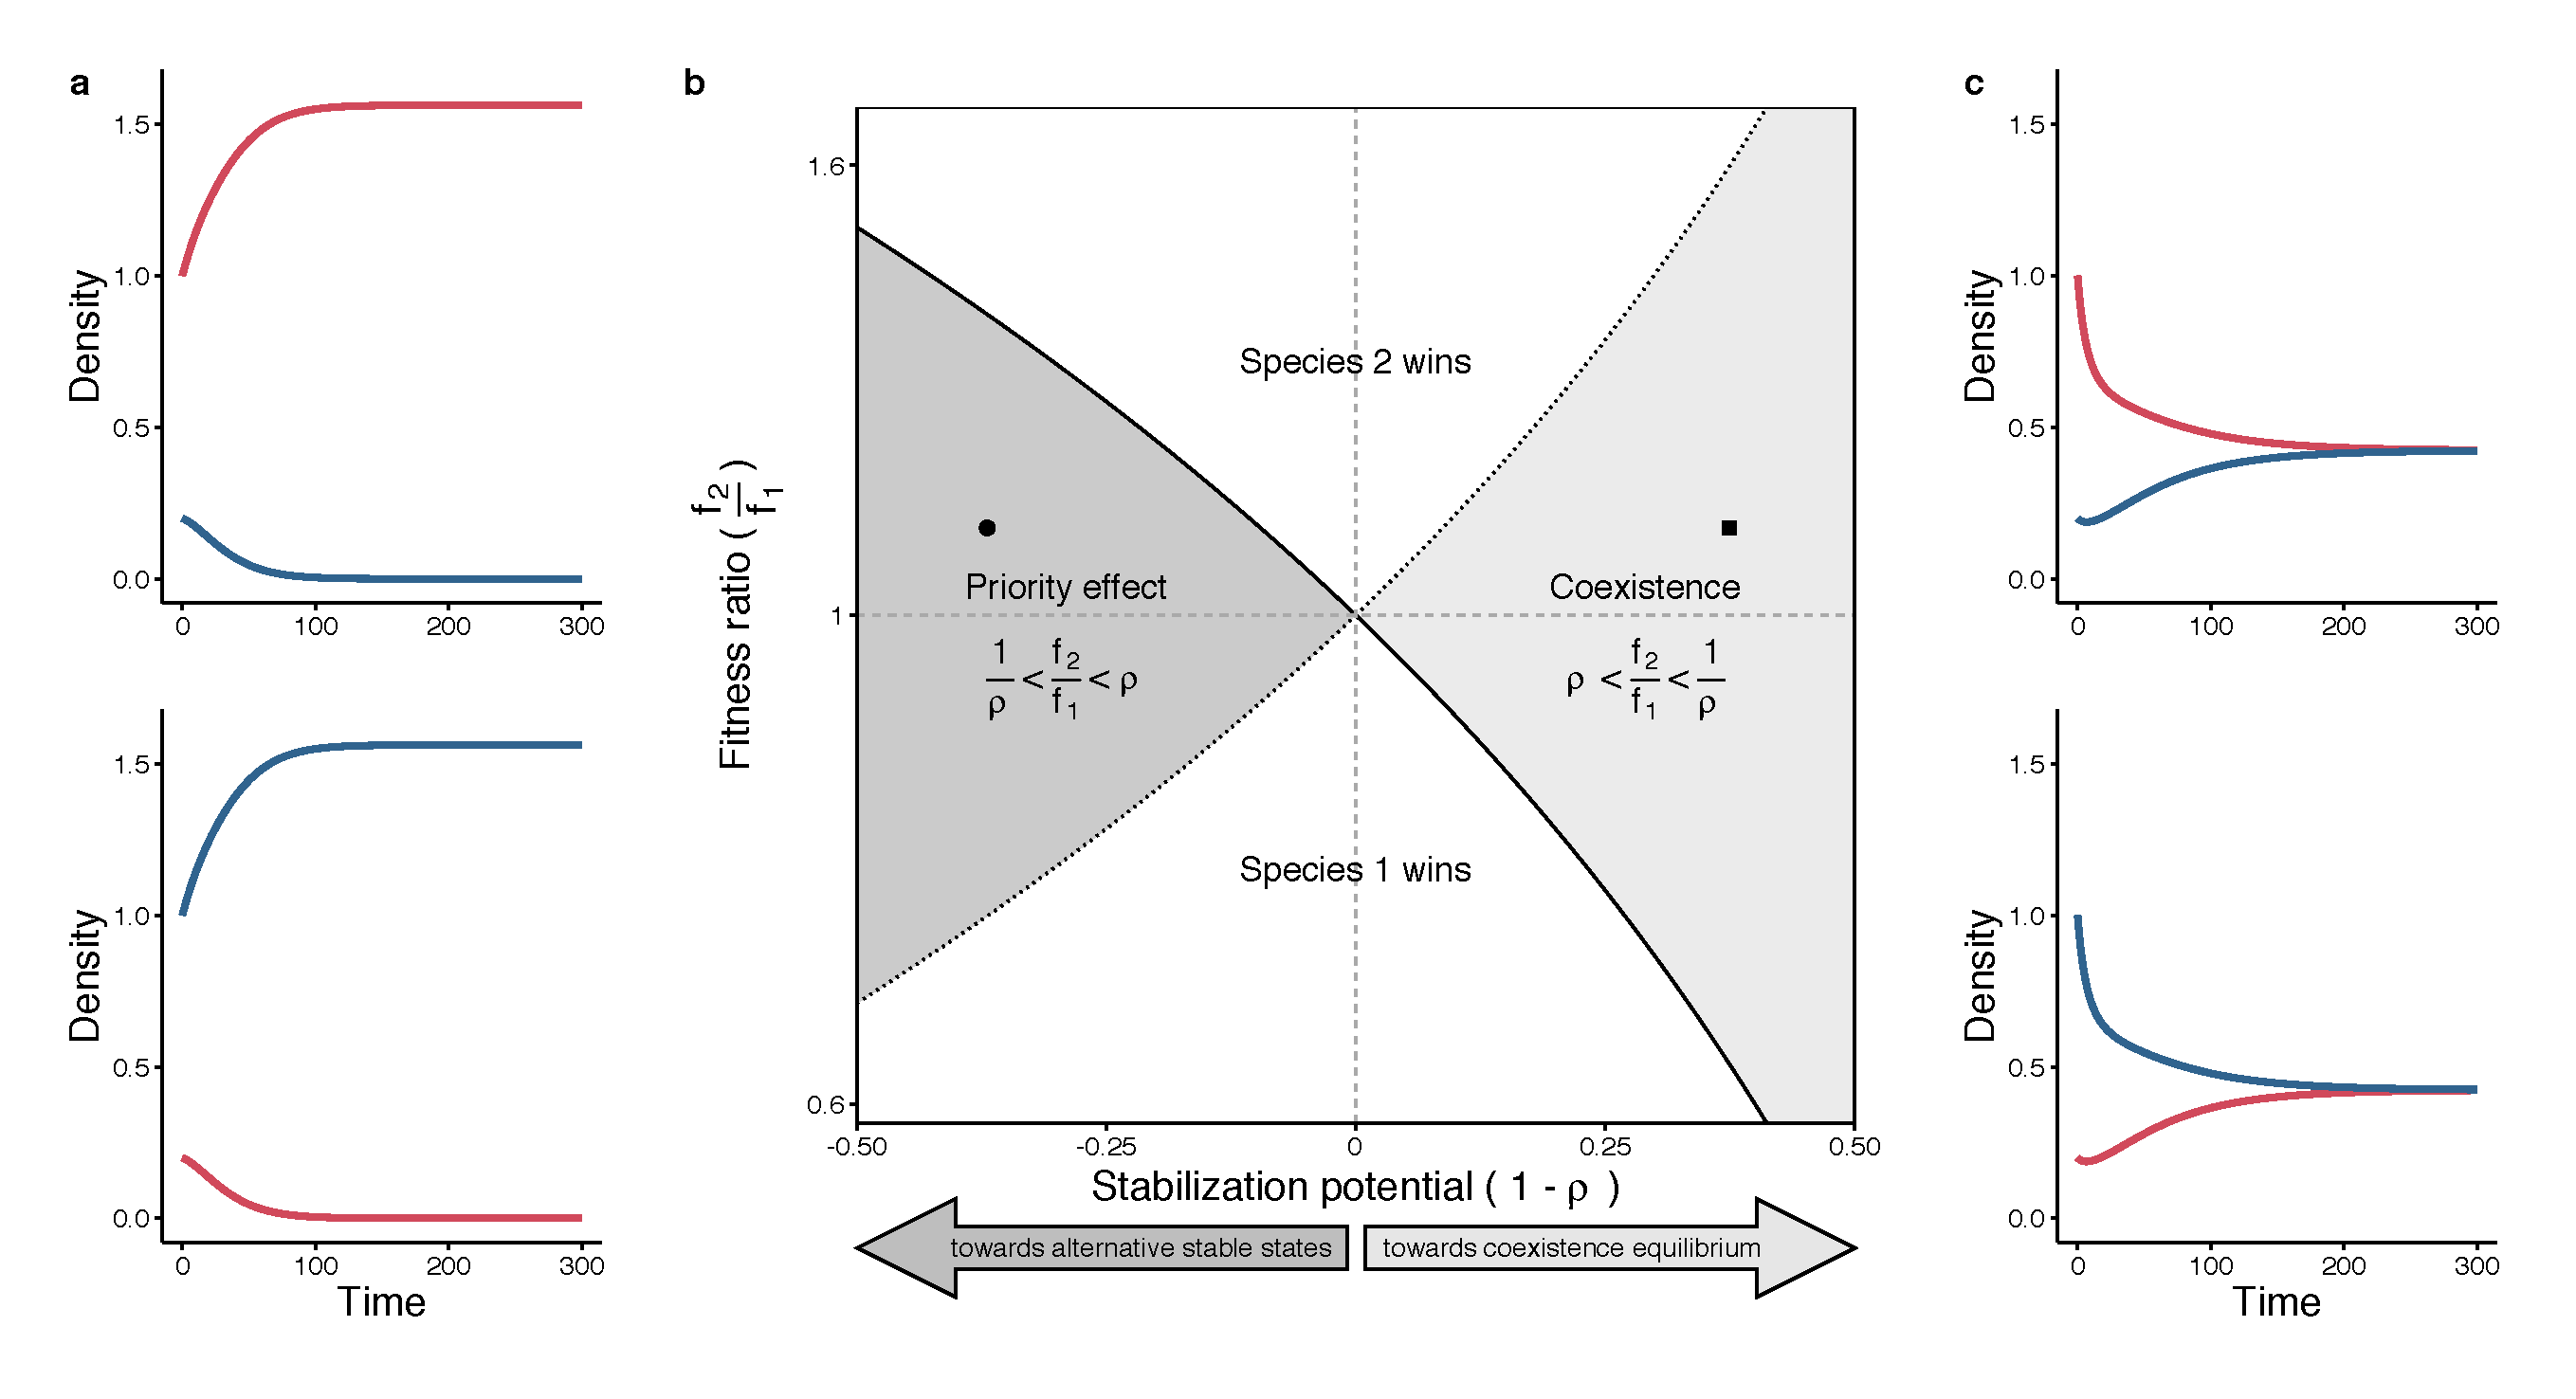
\includegraphics[width=14cm]{Chapter3/Conceptual.pdf}}
	\caption[Coexistence and priority effects in a Lotka--Volterra competition model.]
		{\hspace{1mm}Coexistence and priority effects in a Lotka--Volterra competition model. The community trajectories demonstrating priority effects (a) and stable coexistence (c) correspond to the position of the black circle and black square, respectively, in the central panel (b). In panel (b), the x-axis represents the stabilization potential (1 - $\rho$) and the y-axis represents the fitness ratio, $f_{2}/f_{1}$; the solid and dotted line represents the boundary where $f_{2}/f_{1}$ equals to $\rho$ and $1/\rho$, respectively. The upper and lower white area indicates the region where parameter combinations result in the dominance of species 2 (blue) and 1 (red), respectively; the right light gray and the left dark gray area indicates regions of stable coexistence and priority effects (parameter values and starting values provided in Appendix B).}
	\label{fig:FigBox}
\end{figure}



\newpage
\begin{figure}[h!]
	\centering
	\makebox[\textwidth][c]{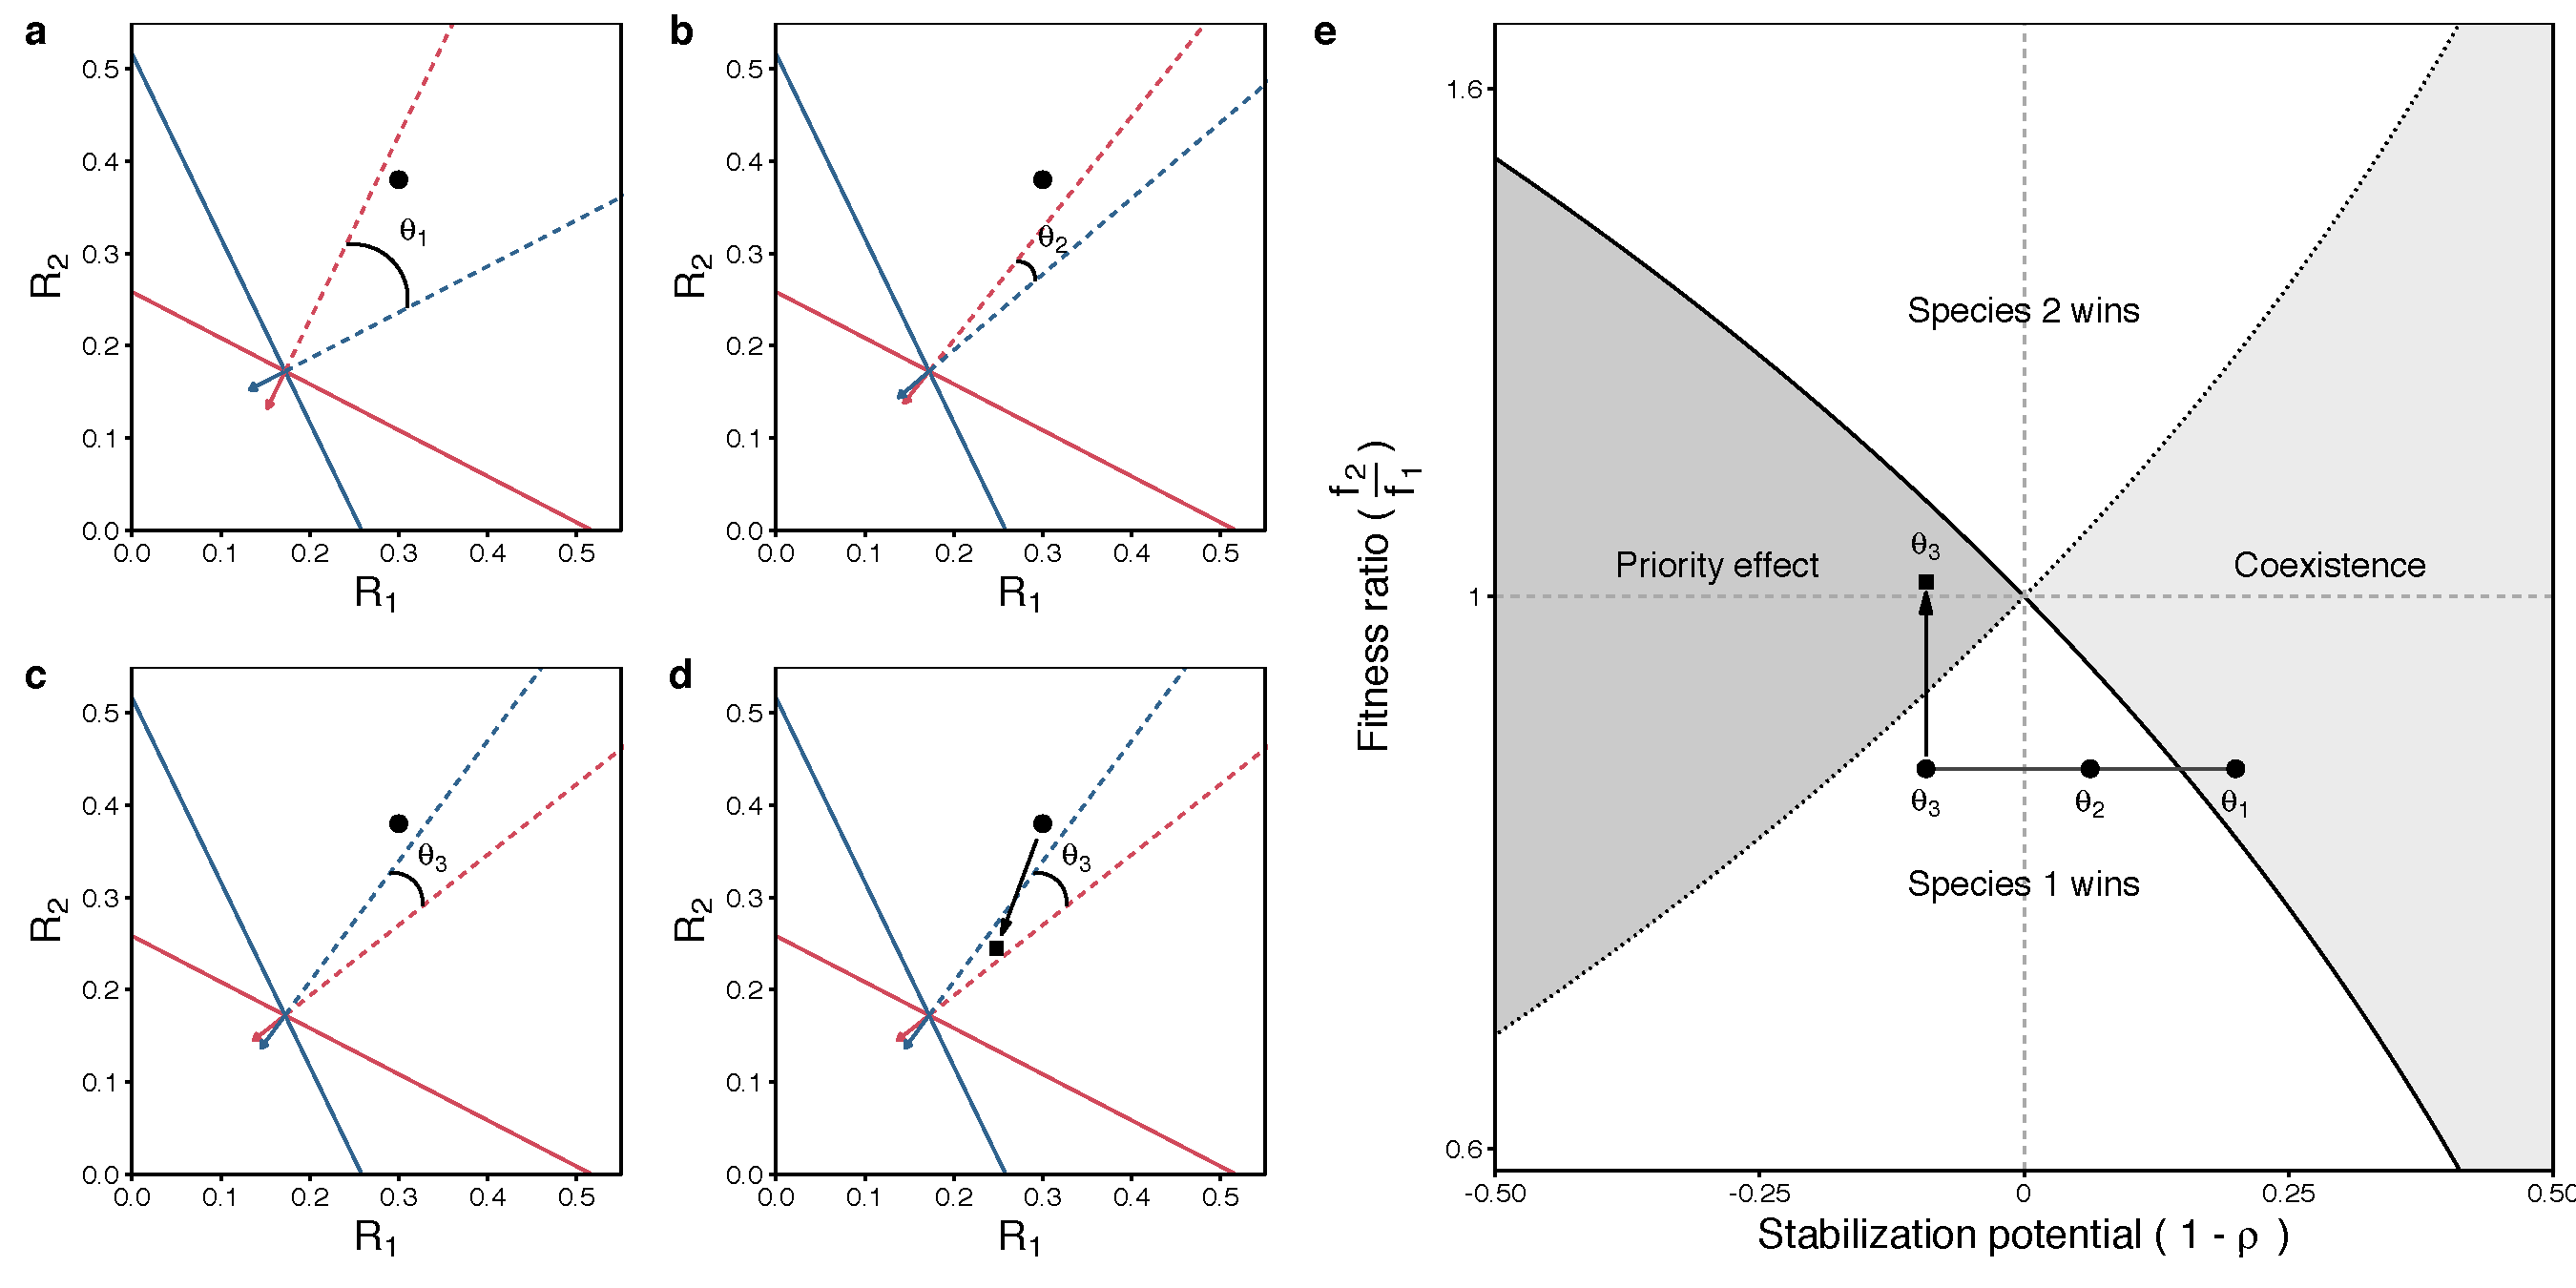
\includegraphics[width=14cm]{Chapter3/Fig1.pdf}}
	\caption[Effect of changing species' consumption vector and the supply ratio of two resources in a consumer-resource model on the fitness ratio and stabilization potential of coexistence theory.]
		{\hspace{1mm}Effect of changing species' consumption vector and the supply ratio of two resources in a consumer-resource model on the fitness ratio and stabilization potential (niche difference) of coexistence theory. In panel (a), the solid red and blue lines are the zero net growth isocline for each species (i.e., species 1 and 2, respectively); the solid lines with arrow heads are the respective consumption vectors; the dashed lines are the inverse of the vectors; and the black circle and square represent two different resource supply ratios (see footnote for technical definition of terms). In panel (a) -- (d), the red species benefits more from consuming $R_{2}$, while the blue species benefits most from $R_{1}$, as indicated by its lower $R^{*}$. In panel (e), the x-axis represents the stabilization potential (1 - $\rho$) and the y-axis represents the fitness ratio, $f_{2}/f_{1}$; and the right and left gray shaded area indicates the coexistence and priority effect region, respectively. The angles given by $\theta_{1-3}$ in panel (a) -- (d) correspond to the respective $\theta_{1-3}$ in panel (e). Note that the y-axis is on log-scale. Analytical treatment and simulation parameters provided in Appendix B.}
	\label{fig:Fig1}
\end{figure}



\newpage
\begin{figure}[h!]
	\centering
	\makebox[\textwidth][c]{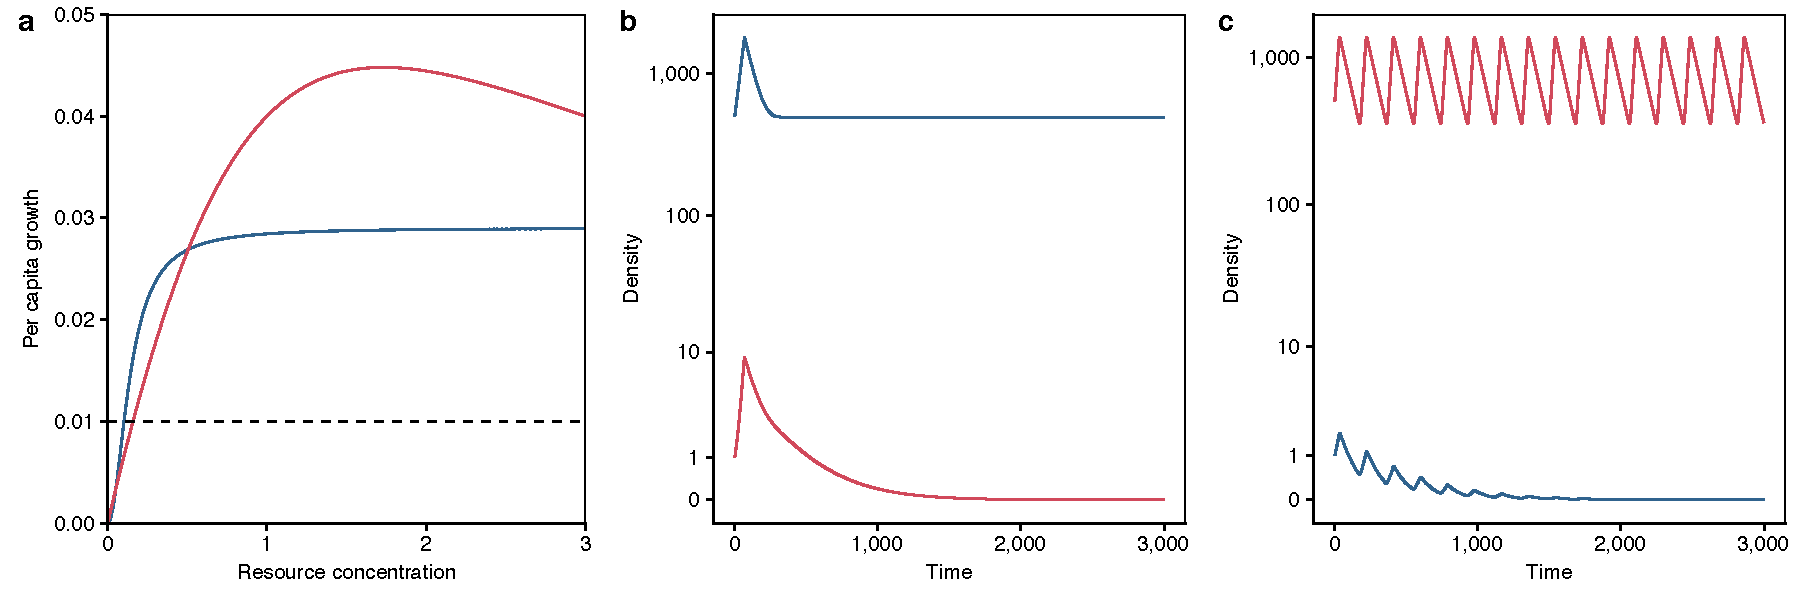
\includegraphics[width=14cm]{Chapter3/relnonlin.pdf}}
	\caption[Positive frequency dependence emergeing from endogenously generated resource fluctuations.]{\hspace{1mm}Positive frequency dependence emerges from endogenously generated resource fluctuations. In panel (a), blue is the better competitor at low resource levels and also suppresses fluctuations in the resource to its own advantage; Red is the better competitor at moderate resource levels, and, because of a highly nonlinear functional response owing to inhibited growth at high resource levels, generates fluctuations in the resource to its own advantage. Provided each species begins at a sufficiently higher density than its competitor, it is able to prevent its competitor from invading (b, c). Simulation parameters provided in Appendix B.}
	\label{fig:Fig2}
\end{figure}



\newpage
\begin{tcolorbox}[breakable, colback=white, leftright skip=-0.5cm]
	\label{fig:Box}
	\subsubsection*{Box 1 -- Coexistence and priority effects in a Lotka--Volterra competition model}
	Whether coexistence or priority effects emerges in a two-species Lotka--Volterra competition model depends on the relative magnitude of intra- and inter-specific competition. Consider the following Lotka--Volterra model:
	\begin{align*}
	\frac{dN_{1}}{dt}=r_{1}N_{1}\left ( 1-a_{11}N_{1}-a_{12}N_{2} \right ), \tag{3.5}\label{eq:LV1}
	\\~\\
	\frac{dN_{2}}{dt}=r_{2}N_{2}\left ( 1-a_{21}N_{1}-a_{22}N_{2} \right ). \tag{3.6}\label{eq:LV2}
	\end{align*}
	Each species intrinsic growth rate, $r_{1}$ and $r_{2}$, is negatively affected by intra-specific ($\alpha_{11}$ and $\alpha_{22}$) and inter-specific competition ($\alpha_{12}$ and $\alpha_{21}$). The two species stably coexist with positive densities if $\alpha_{11} > \alpha_{21}$ and $\alpha_{22} > \alpha_{12}$; that is, when intra-specific competition exceeds inter-specific competition. Under this scenario, each species exhibits negative frequency dependence since an increase in its abundance leads to larger negative impact on itself. Alternatively, when inter-specific effects exceed intra-specific effects, i.e., $\alpha_{11} < \alpha_{21}$ and $\alpha_{22} < \alpha_{12}$, each species exhibits positive frequency dependence; an increase in its abundance results in a larger negative impact on the competitor. This leads to priority effects in the form of alternative stable states. The community trajectory is attracted to one of the two monoculture equilibriums, dominated by either $N_{1}$ or $N_{2}$, depending on the initial abundance of the two species.
	\par
	
	
	The relationship between $\alpha_{ij}$'s and competition outcomes can be directly mapped onto the parameter space of the stabilization potential (1 - $\rho$, x-axis) and the fitness ratio ($f_{2}/f_{1}$, y-axis) (panel b of Fig.~\ref{fig:FigBox}, see main text). The solid ($f_{2}/f_{1} = \rho$) and dotted ($f_{2}/f_{1} = 1/\rho$) boundaries partition the parameter space into four distinct regions, each representing different outcomes of competition. The light gray area on the right ($\rho < \frac{f_{2}}{f_{1}} < 1/\rho$) indicates parameter combinations that result in stable coexistence. This requires $\rho$ to be bounded between zero and one, which is guaranteed when intra-specific competition is stronger than inter-specific competition. The dark gray area on the left ($1/\rho < \frac{f_{2}}{f_{1}} < \rho$) indicates the parameter space such that $\rho$ is greater than one, resulting in priority effects. 
\end{tcolorbox}
